\section{In-house statistical debugging}
\label{sec:inhouse}
During in-house performance diagnosis, users send detailed bug reports to
the developers and developers often repeat the performance problems
observed by the users before they start debugging.
Following the study in Section \ref{sec:study}, this section designs and
evaluates statistical debugging for in-house diagnosis of real-world
performance problems.
We aim to answer three key questions.

\begin{enumerate}
\item What statistical debugging design is most suitable for diagnosing
real-world performance problems;
\item What type of performance problems can be diagnosed by statistical
debugging;
\item What type of performance problems cannot be diagnosed by statistical
debugging alone.
\end{enumerate}

\subsection{Design}
In general, statistical debugging 
\cite{liblit03,liblit05,CCI,tarantula1,tarantula2,tarantula.darko,joy.asplos13}
is an approach that uses statistical machine learning techniques to help
failure diagnosis. It usually works in two steps.
First, a set of run-time 
events $E$ are collected from both success runs and failure runs.
Second, a statistical model is applied to identify an event $e \in E $
that is most correlated with the failure, referred to as the failure predictor. 
Effective statistical debugging can identify failure predictors that are
highly related to failure root causes and help developers fix the underlying
software defects.

There are three key questions in the design of statistical debugging.
\begin{enumerate}
\item Input design --
what inputs shall we use to drive the 
incorrect execution and the correct execution during statistical debugging.
If the good runs and the bad runs are completely different
(e.g., they do not cover any common code regions), the diagnosis will
be difficult.
\item Predicate design -- what type of run-time events shall we monitor.
Roughly speaking, a predicate $P_i$ could be true or false, depending on 
whether a specific property is satisfied at instruction $i$ at run time.
To support effective diagnosis, one should choose predicates that can reflect 
common failure root causes.
\item Statistical model design -- what statistical model shall we use to
rank predicates and identify the best failure predictors among them.
\end{enumerate}

The input design problem is naturally solved for performance diagnosis, as
discussed in Section \ref{sec:study}. We discuss different predicate designs
and statistical model designs below.

\subsubsection{Predicate designs}
Many predicates have been designed to diagnose functional bugs.
We discuss some commonly used ones below.

\paragraph{Branches.} There are two branch 
predicates associated
with each branch $b$: one is true when $b$ is taken, and the other is true when
$b$ is not taken \cite{liblit03,liblit05}.

\paragraph{Returns.} There are a set of six return predicates
for each function return point, tracking whether the return value is ever
$<0$, $\leq 0$, $>0$, $\geq 0$, $=0$, or $\neq 0$ \cite{liblit03,liblit05}.
%negative, zero, or positive \cite{liblit03,liblit05}.

\paragraph{Scalar-pairs.} There are six scalar-pair predicates
for each pair of variables $x$ and $y$, tracking whether $x$ is ever 
$<y$, $\leq y$, $>y$, $\geq y$, $=y$, or $\neq y$ \cite{liblit03,liblit05}.
%smaller than,
%larger than, or equal to $y$ \cite{liblit03,liblit05}. 
Whenever a scalar
variable $x$ is updated, scalar-pair predicates are evaluated between $x$ and
each other same-type variable $y$ that is in scope, as well as program 
constants.

\paragraph{Instructions.} Instruction predicate $i$ is true, if 
$i$ has been executed during the monitored run 
\cite{tarantula1,tarantula2,tarantula.darko}.

\paragraph{Interleaving-related ones.} Previous work on diagnosing
concurrency bugs \cite{CCI} has designed three types of predicates that are 
related to
thread interleaving. For example, CCI-Prev predicates track whether two 
consecutive accesses to a
shared variable come from two distinct threads or the same thread.

In the remainder of this section, we will focus on three predicates: branch
predicates, return predicates, and scalar-pair predicates. We skip
instruction predicates in this study, because they are highly related to
branch predicates. We skip interleaving-related predicates in this study,
because most performance problems that we study are deterministic and
cannot be effectively diagnosed by interleaving-related 
predicates.

\begin{table*}
  \centering
  \small
  \newcommand{\Yes}[1]{\checkmark{}$_#1$}
  \newcommand{\No}[0]{-}
  \begin{tabular}{lccccccc}
    \toprule
              &          &         & \multicolumn{3}{c}{\bf Static \# of predicates}& {\bf Static \# of} & {\bf Reported Inputs}\\
    \cmidrule(lr){4-6}
     {\bf BugID}     &{\bf KLOC}   &{\bf Language}    &{\bf Branch}    &{\bf Return}   &{\bf Scalar-pair}   &{\bf Loops}    &{\bf (bad/good)} \\
    \midrule
    Mozilla258793    & 3482        & C++              & 385722         & 1126770       & *                & 10016         & n/0            \\
    Mozilla299742    & 3482        & C++              & 385720         & 1126698       & *                & 10016         & 1/0            \\
    Mozilla347306    & 88          & C                & 26804          & 38634         & 271968             & 951           & n/n            \\
    Mozilla416628    & 105         & C                & 28788          & 39306         & 302496             & 1420          & 1/0            \\
    \midrule
    MySQL15811       & 1149        & C++              & 13508          & 15576         & *                & 760           & n/n            \\
    MySQL26527       & 986         & C++              & 90128          & 128610        & *                & 4222          & n/n            \\
    MySQL27287       & 995         & C++              & 92316          & 119322        & *                & 4683          & n/n            \\
    MySQL40337       & 1191        & C++              & 103686         & 138582        & *                & 4510          & n/n            \\
    MySQL42649       & 1164        & C++              & 126822         & 155766        & *                & 5688          & n/n            \\
    MySQL44723       & 1164        & C++              & 126822         & 155766        & *                & 5688          & 1/1            \\
    \midrule
    Apache3278       & N/A         & Java             & 10             & 126           & 204                & 7             & n/n           \\
    Apache34464      & N/A         & Java             & 22             & 42            & 342                & 8             & n/n           \\
    Apache47223      & N/A         & Java             & 24             & 36            & 390                & 9             & n/n           \\
    Apache32546      & N/A         & Java             & 6              & 66            & 120                & 5             & n/n           \\
    \midrule
    GCC1687          & 2099        & C                &  183496 & 296058 & 4187586 & 6476     & n/n            \\
    GCC8805          & 2538        & C                &  207188 & 327804 & 4161012 & 7309     & n/n            \\
    GCC15209         & 2586        & C                &  192108 & 304800 & 3705558 & 7310     & 1/1            \\
    GCC21430         & 3844        & C                &  238514 & 447510 & 3768078 & 9078     & n/n            \\
    GCC46401         & 5521        & C                &  337810 & 713532 & 5625606 & 15159    & 1/1            \\
    GCC12322         & 2341        & C                &  177098 & 284484 & 3750912 & 6563     & 1/0            \\
    \bottomrule
   \end{tabular}
  \nocaptionrule
  \caption{Benchmark information. (N/A: since our statistical debugging tools 
      only work for C/C++ programs, we have 
	reimplemented the four Java benchmarks in C programs. *: we have no
	tools to collect scalar-pair predicates in C++ programs. 
	The 1s and $n$s in the
	``Reported Inputs'' column indicate how many bad/good inputs are reported
	by users.)}
  \label{tab:benchmarks}
\end{table*}

\subsubsection{Statistical model designs}
Many statistical models have been used before for anomaly 
detection \citep{engler01bugs,CPMiner04,kremenek06inferring,lamsigsoft02} 
and fault localization 
\citep{liblit03,liblit05,CCI,tarantula1,tarantula2,tarantula.darko,Delta-LDA}.
Although the exact models used by previous work differ from each other, they 
mostly follow the same principle --- if a predicate is a good failure predictor,
it should be true in many failure runs, and be false or not-observed
in many success runs. They can be roughly categorized into two classes.
The first class
only considers whether a predicate has been observed
true for at least once in a run (e.g., whether a branch $b$ has been
taken for at least once). The exact number of times the predicate has
been true in each run is not considered in the model.
The second class instead considers the exact number of times a predicate has 
been true in each run.
Naturally, by considering more information in the model, the second class could
complement the first class, but at the cost of longer processing time.
Most previous work on functional bug
diagnosis has found the first class sufficient 
\cite{liblit03,liblit05,CCI,joy.asplos13} and did not try 
the second class.

To cover both classes of statistical models for performance diagnosis, our 
study will look at two models: a
\emph{basic} model proposed by CBI work \citep{liblit03,liblit05} that belongs
to the first class discussed above 
and a $\Delta$LDA model proposed by \citet{Delta-LDA} that belongs
to the second class discussed above. 
We leave investigating other existing statistical
models and designing new models to future work. Since our evaluation will use
exactly the same formulas, parameters, and settings
for these two models as previous work \citep{liblit03,liblit05,Delta-LDA}, we
briefly discuss these two models below.
More details about these two models can be found in their
original papers \citep{liblit03,liblit05, Delta-LDA}. 

\paragraph{Basic model}
This model works in two steps.
First, it checks whether an execution is more likely to fail 
when a predicate $P$ is observed true, 
whose probability is computed by formula \textit{Failure}$(P)$, 
than when $P$ has merely being observed during the execution, 
whose probability is computed by formula \textit{Context}$(P)$.
Consequently, only predicates, whose \textit{Increase} values computed below
are higher than 0 with
certain statistical confidence, will appear in the final ranking list.
By default, statistical Z-tests and 0.99 confidence level are 
used in CBI \cite{liblit03}.

\[
Failure(P) =  \frac{F(P_{\text{true}})}{S(P_{\text{true}})+F(P_{\text{true}})}
\]

\[
Context(P) =  \frac{F(P_{\text{observed}})}{S(P_{\text{observed}})+F(P_{\text{observed}})}
\]

\[
Increase(P) =  Failure(P) - Context(P)
\]

$F(P_{\text{true}})$ is the number of failure runs in which P is true, 
and $F(P_{\text{observed}})$
is the number of failure runs in which P is observed, no matter true or false. 
$S(P_{\text{true}})$ is the number of success runs 
in which P is true, and $S(P_{\text{observed}})$
is the number of success runs in which P is observed. 

 
\[
Importance(P) =  \frac{2}{\frac{1}{Increase(P)} + \frac{1}{log(F(P_{\text{true}}))/log(F)}}
\]

The final ranking is based on an \textit{Importance} metric. This metric
reflects the harmonic mean of
the \textit{Increase} metric and the conditional probability of a predicate $P$
being true given that an execution has failed. 
$F$ is the total number of failure runs in the formula above.
Previous work 
\cite{liblit05}
has tried different
variants of the harmonic mean and found the formula above, with a logarithmic
transformation, to be the best. As mentioned above, we reuse all the formulas, 
parameters, and settings from previous work. 

\paragraph{$\Delta$LDA model}
$\Delta$LDA~\cite{Delta-LDA} model is derived from a famous machine learning
model, called Latent Dirichlet Allocation 
(LDA) \cite{LDA}.
By considering how many times a predicate is true 
in each run, it can pick up weaker bug signals, as shown by previous work \cite{Delta-LDA}.
Imagine the following scenario ---
during a success run, predicate $P$ is true for
10 times and false for 100 times; during a failure run, $P$ is true for 
100 times and false for 10 times. The basic model will consider $P$ as useless,
as it has been observed both true and false in every run. However, $\Delta$LDA model will 
notice that $P$ is true for many more times during each failure run than that in 
each success
run, and hence consider $P$ as failure predictor. The exact ranking formula of
$\Delta$LDA model is very complicated, and is skipped here. It can be found
in previous work \cite{Delta-LDA}.
  
\paragraph{How to apply the models}
A statistical debugging framework collects the following
information from each run: (1) whether the run has succeeded and failed;
%(2) a list of predicates that have been observed and for how many times each
%(the latter only for $\Delta$LDA model); 
(2) a list of predicates that have been observed true and for how many 
times each (the latter only for $\Delta$LDA model). 
After collecting such information from
several success runs and failure runs, the framework will naturally obtain
values, such as the number of failure runs where a predicate is observed/true,
for the formulas discussed above and produce a rank list of failure predictors.




\subsection{Experimental evaluation}
\label{sec:inhouse_results}
\subsubsection{Methodology}
\label{sec:inhouse_meth}
To evaluate how statistical debugging works for real-world performance problems,
we apply three types of predicates and two types of statistical models on 
real-world user-reported performance problems.
All our experiments are conducted on an Intel i7-4500U machine, with Linux 3.11 kernel.

\paragraph{Benchmark selection}
Among the 65 user-reported performance problems discussed in Section 
\ref{sec:study}, we have tried our best effort and successfully repeated 20
of them from four different C/C++/Java 
applications. In fact, most of the 65 performance problems are deterministically repeatable based on the bug reports.
We have failed to repeat 45 of them for this
study mainly because they depend on special hardware platforms or very
old libraries that are not available to us or very difficult to set up. 
The detailed information for the 20 performance problems used in our experiments 
is shown in Table~\ref{tab:benchmarks}.
Specifically, the static number of branch predicates is counted based on the 
fact that
there are two predicates for each static branch instruction in the user program
(excluding library code). The static numbers of other predicates are similarly
counted.
%For C (and Java) benchmarks, CBI will count these three numbers and put them in the final results automatically. 
%For C++ benchmarks, the number of branch predicates is the product of 2 
%and the number of conditional branch instruction inside each binary code, 
%and the number of return predicates is the product of 6 
%and the number of call sites whose return types are characters, 
%integers or pointers inside each binary code. 
%These are following the same instrumentation scheme inside CBI. 
%The 7th column shows the number of static loops inside each compiled binary code. 
%We get numbers in this column by implementing a simple counting tool based on Dyninst~\cite{dyninst}. 

To make sure these 20 benchmarks are representative, we also conduct
manual source-code inspection to see how statistical debugging could work
for \textbf{all} the 65 user-reported performance problems in our study. 
We will show that our
manual inspection results on all the 65 cases are \textbf{consistent} with
our experimental evaluation on these 20 benchmarks. 

%{\bf [Linhai also checked profiling ranks for functions containing the final patches. 
%For 7 bugs, functions containing final patches are not shown in the profiling ranking
%lists. For the rest of 13 bugs, the median of ranks for functions containing final patches is 19. ]}
%




\paragraph{Input design}
To conduct the statistical debugging, we run each benchmark program 20 times, using
10 unique good inputs and 10 unique bad inputs.
For each performance problem, we get its corresponding 20 inputs based on users'
bug report. For 13 of them, the bug reports have described
how to generate a large number of good and bad inputs, which makes our input
generation straightforward. For the remaining 7 bugs, with 3 from Mozilla, 3 
from GCC, and 1 from MySQL, we randomly
change the provided inputs and use the user-provided failure-symptom
information to decide which inputs are good or bad.
We make sure that inputs generated by us are still valid HTML webpages, valid JavaScript programs,
valid C programs, or valid database tables/queries.
The process of judging which inputs
are good or bad is straightforward,
as discussed in Section \ref{sec:study_imp}.
For example, Mozilla\#299742 reports a webpage that leads to a consistent
CPU usage rate above 70\%, while some similar webpages lead to less than 10\% 
CPU usage rate. We generate many inputs by randomly replacing some content of this 
webpage with content from other randomly picked webpages, and judge whether
the inputs are good or bad based on CPU usage. 

\paragraph{Techniques under comparison}
We will evaluate three predicates (branches, returns, scalar-pairs)
and two statistical models (basic, $\Delta$LDA) for statistical debugging.
For C programs, we use CBI \cite{liblit03,liblit05} to collect all these
three types of predicates\footnote{
CBI~\cite{liblit03,liblit05} 
is a C framework for lightweight instrumentation and statistical debugging. 
It collects predicate information from both success and failure runs,
and utilize statistical 
model to identify the likely causes of software failures. 
}.
For C++ programs, we implement our own branch-predicate and
return-predicate collection tools using
PIN binary-instrumentation framework \cite{pin}.
Scalar-pair predicates are very difficult to evaluate using PIN, 
and hence are skipped for C++ programs in our experimental evaluations.
They will be considered for all benchmarks in our manual study 
(Section \ref{sec:manual_results}).
Since the exact execution time is not the target of our information collection,
we did not encounter any observer effect in our experiment.

We use the default settings of the CBI basic model and the 
$\Delta$LDA model for \textit{all} the benchmarks in our evaluation.
Specifically, CBI model only has one parameter --- the statistical
confidence level for filtering out predicates based on the \textit{Increase}
metric. We use the default setting 0.99. The key parameter
in $\Delta$LDA model is the number of bad topics. We use the default setting
1.

We also use \textit{OProfile} \cite{oprofile} to get profiling results in our 
experiments.
We provide two types of profiling results, both of which are under the
``Profiler'' column in Table \ref{tab:in-house}.
``Fun'' demonstrates where the root-cause function ranks in the profiler 
result and what is the distance between 
the root-cause function and where patches are applied. 
``Stack'' considers the call-chain information provided by OProfile for each function
in its ranking list. It first checks whether any direct or indirect caller functions
of the top OProfile-ranked function is related to the root
cause; if not, it then checks the callers, callers' callers, and so on
of the second top ranked function;
and so on.
Among the 65 bug reports in our study, 13 of them mentioned the use of 
profilers. Among these 13, 4 of them mentioned the use of call-chain information
provided by the profilers.
%OProfile can only provide correct caller-callee information for applications 
%built with enabling frame pointers. 
%Data under ``Fun'' column is got from application under default building settings, 
%and data under ``Stack'' column is from application built with frame pointers enabled. 
For the simplicity of explanation, we will use the ``Fun'' setting as the
default setting for discussing profiler results,
unless specified otherwise.
%The average overhead of applying OProfile on each benchmark under bad inputs
%are shown in the second-to-last column in Table \ref{tab:benchmarks}.
\comment{
The ``Profiler'' column in Table \ref{tab:in-house}
will show where the root-cause function ranks in the profiler result
and what is 
the distance between the root-cause function
and where patches are applied.
} 
%When the top-ranked function is in the same file as the patch, we 
%count the distance between the patch and the function entrance or exit, 
%whichever is closer.
%When the top-ranked function is in a different file from the patch, we
%mark the distance as
%$.$. 

\begin{table*}
  \centering
  \footnotesize
  \newcommand{\Yes}[1]{\checkmark{}$_#1$}
  \newcommand{\Yess}[0]{\checkmark{}}
  \newcommand{\No}[0]{-}
  \begin{adjustwidth}{-.25in}{-.25in}
  {
  \begin{tabular}{lcccccccccccl}
    \toprule
                 &\multicolumn{3}{c}{\# of candidate predicates}& \multicolumn{3}{c}{Basic model}& \multicolumn{3}{c}{$\Delta$LDA model}&\multicolumn{2}{c}{Profiler}&Developers' fix strategy\\
\cmidrule(lr){2-4}
\cmidrule(lr){5-7}
\cmidrule(lr){8-10}
\cmidrule(lr){11-12}
    {\bf BugID}    & {Branch} & {Return} & {S-pair} & {Branch}    & {Return}    & {S-pair}   & {Branch$_{\text{loop}}$}     &  {Return}  & {S-pair}   & Fun         & Stack            &\\
    \midrule
    Mozilla258793  &  62822   & 149354   &  *       & \Yes{1}(0)  & \No         &  *         & \No          &  \No       &  *         & \No         &\No            & Change branch condition\\
    Mozilla299742  &  61256   & 148688   &  *       & \Yes{1}(0)  & \No         &  *         & \No          &  \No       &  *         & \No         &\No            & Change branch condition\\
    Mozilla347306  &   3931   & 4062     &  21590   & \No         & \No         & \No        & \Yes{1}(1)   & \Yes{1}(1) &\Yes{1}(1)  & \Yes{1}(7)  &\Yess$_{1[0]}$  & Remove the loop\\
    Mozilla416628  &   3719   & 3598     &  19428   & \No         & \No         & \No        & \Yes{1}($.$) &  \No       &\Yes{1}($.$)& \Yes{1}($.$)&\Yess$_{1[0]}$  & Reduce \# loop iterations\\
    \midrule                                                                                                         
    MySQL15811     &   1198   & 866      &  *       & \No         & \No         &    *       & \Yes{1}($.$) &\Yes{1}(0)  &  *         & \Yes{1}($.$)&\Yess$_{1[0]}$  & Remove the loop\\
    MySQL26527     &   6422   & 6823     &  *       & \Yes{1}(0)  & \No         &  *         & \No          & \No        &  *         & \No         &\No            & Change branch condition\\
    MySQL27287     &   5377   & 5752     &  *       & \No         & \No         &  *         & \Yes{1}(0)   & \No        &  *         & \Yes{1}(0)  &\Yess$_{1[0]}$  & Remove the loop\\
    MySQL40337     &   7868   & 8160     &  *       & \Yes{1}(1)  & \No         &  *         & \No          & \No        &  *         & \No         &\No	    & Change branch condition\\
    MySQL42649     &  12569   & 9696     &  *       & \Yes{1}($.$)& \No         &  *         & \No          & \No        &  *         & \No         &\No            & Optimize branch body\\
    MySQL44723     &  10476   & 9108     &  *       & \Yes{1}($.$)& \No         &  *         & \No          & \No        &  *         & \No         &\Yess$_{1[2]}$  & Optimize branch body\\
    \midrule                                                                                                         
    Apache3278     &  7       & 63       & 102      & \Yes{1}(3)  & \Yes{1}(2)  & \Yes{1}(2) & \No          & \No        & \No        & \No 	    &\No	    & Synchronization adjustment\\
    Apache34464    &  17      & 23       & 193      & \No         & \No         & \No        & \Yes{3}(0)   & \Yes{1}(2) & \No        & \Yes{5}(2)  &\Yess$_{1[1]}$  & Combine loop instances\\
    Apache47223    &  17      & 15       & 237      & \No         & \No         & \No        & \Yes{1}($.$) & \No        &\Yes{1}($.$)& \Yes{1}($.$)&\Yess$_{1[0]}$  & Combine loop instances\\
    Apache32546    &  5       & 34       & 69       & \No         & \No         & \No        & \Yes{1}(8)   & \Yes{1}(7) & \Yes{1}(7) & \No         &\Yess$_{5[0]}$  & Combine loop iterations\\
    \midrule                                                                                                         
    GCC1687        & 22602    & 17787    & 428103   & \No         & \No         & \No        & \Yes{1}($.$) &\Yes{2}($.$)&\No         & \Yes{1}($.$)&\checkmark{}$_{1[0]}$ & Combine loop iterations\\ 
    GCC8805        & 23891    & 20467    & 404594   & \No         & \No         & \No        & \Yes{4}(0)   &\Yes{1}(0)  &\No         & \No         &\No	& Reduce \# loop iterations\\ 
    GCC15209       & 8956     & 9403     & 155007   & \Yes{1}(13) & \No         & \No        & \No          & \No        &  \No       & \No  	    &\No	& Change branch condition\\
    GCC21430       & 45494    & 51270    & 647228   & \No         & \No         & \No        & \Yes{1}(0)   & \No        & \Yes{1}(0) & \Yes{1}(2)  &\checkmark{}$_{1[0]}$	& Remove the loop\\ 
    GCC46401       & 34365    & 38263    & 479508   & \No         & \No         & \No        & \Yes{2}($.$) &\Yes{3}($.$)&\Yes{1}($.$)& \Yes{5}($.$)&\checkmark{}$_{1[2]}$ & Reduce \# loop iterations\\ 
    GCC12322       & 46721    & 38269    & 878823   & \No         & \No         & \No        & \No          & \No        &  \No       & \No      &\checkmark{}$_{1[1]}$ & Reduce \# loop iterations\\
    \bottomrule
   \end{tabular}
  }
  \end{adjustwidth}
  \nocaptionrule
  \caption{Experimental results for in-house diagnosis 
    (\Yes{x}(y): the $x$-th ranked failure predictor is highly
     related to the root
     cause, and is $y$ lines of code away from the patch.
     $(.)$: the failure predictor and the patch are more than 50 lines of
     code away from each other or are from 
     different files. 
     \checkmark{}$_{x[y]}$: a $y$-th level caller of 
     the $x$-th ranked
     function in a profiler result is related to the root cause; 
     $_x[0]$ means it is the function itself that is related to the root cause.
     \No: none of the top five predictors
     are related to the root cause or no predicates reach the
     threshold of the statistical model.).}
  \label{tab:in-house}
\end{table*}


\subsubsection{Results for basic model}
\label{sec:inhousebasic}
Overall, 8 out of 20
performance problems can be successfully diagnosed 
using the basic statistical model.
Furthermore, in all these 8 cases, the failure predictor
that is ranked number
one by the
statistical model is indeed highly related to the root cause of the
performance problem. 
Consequently, developers will not waste their time in 
investigating spurious failure predictors.

Among all three types of evaluated predicates, the branch predicate is the most
useful, successfully diagnosing 8 benchmarks.

The scalar-pair predicate and function-return predicate are only useful
for diagnosing one performance problem, as shown in 
Figure \ref{fig:Apache3278}.
In Apache\#3278, users describe that Tomcat could
non-deterministically take about five seconds to shut-down, which is usually
instantaneous. When applied to Tomcat executions
with fast and slow shut-downs, statistical debugging points out that there are
strong failure predictors from all three types of predicates --- 
(1) the \texttt{if(rc==ETIMEDOUT)} branch on line 5 being taken (branch predicate);
(2) the \texttt{pthread\_cond\_timedwait} function returning 
a positive value (function-return predicate);
(3) the value of \texttt{rc} on line 3 after the assignment is larger than its
original value before the assignment 
(scalar-pair predicate)\footnote{CBI does not consider program constants
for its scalar-pair predicates by default, and hence
cannot capture the comparison between \texttt{rc} and \texttt{ETIMEDOUT} here.}.
These three predicates actually all indicate that 
\texttt{pthread\_cond\_timedwait}
times out without getting any signal. 
A closer look at that code region shows that developers initialize
\texttt{notified} too late. 
As a result, another thread
could set \texttt{notified} to be \texttt{true} and issue a signal even
before the \texttt{notified} is initialized to be \texttt{false} on line 1 of
Figure \ref{fig:Apache3278}, causing a time-out in \texttt{pthread\_cond\_timedwait}. 
This problem can be fixed by moving \texttt{notified=false;} earlier.

\comment{
\begin{figure}
\begin{center}
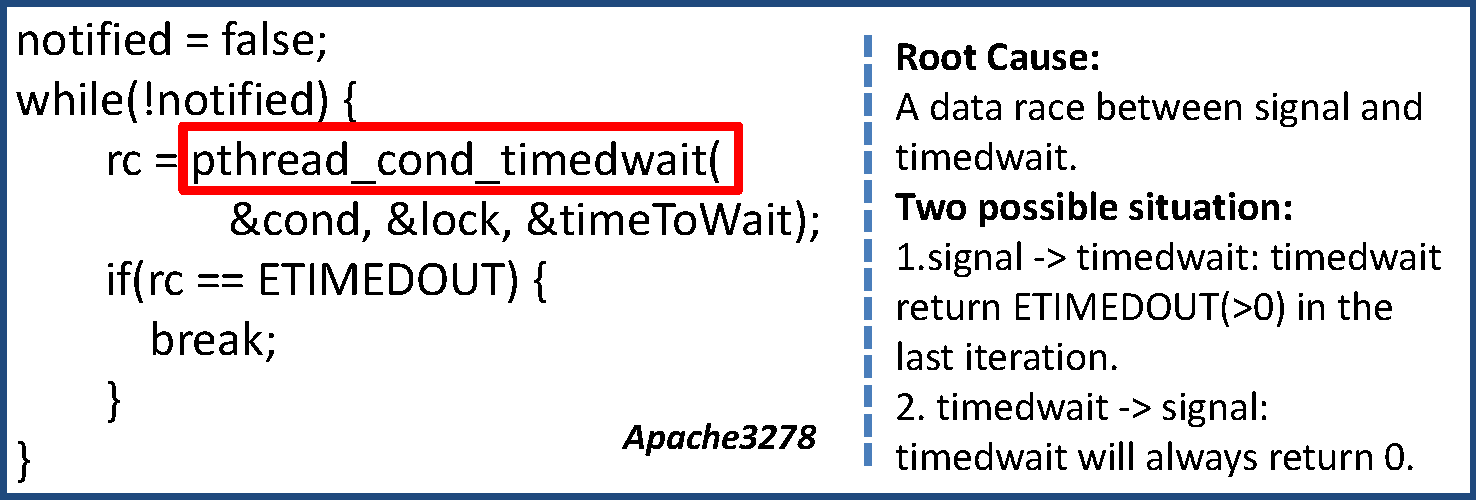
\includegraphics[width=3in]{figures/Apache3278}
\caption{An Apache bug diagnosed by Return}
\label{fig:Apache3278}
\end{center}
\end{figure}
}

\begin{figure}
\centering
\lstinputlisting[basicstyle=\ttfamily\footnotesize,numbers=left]{figures/Apache3278.c}
\caption{An Apache bug diagnosed by Return}
\label{fig:Apache3278}
\end{figure}

\comment{
\begin{figure}
\begin{center}
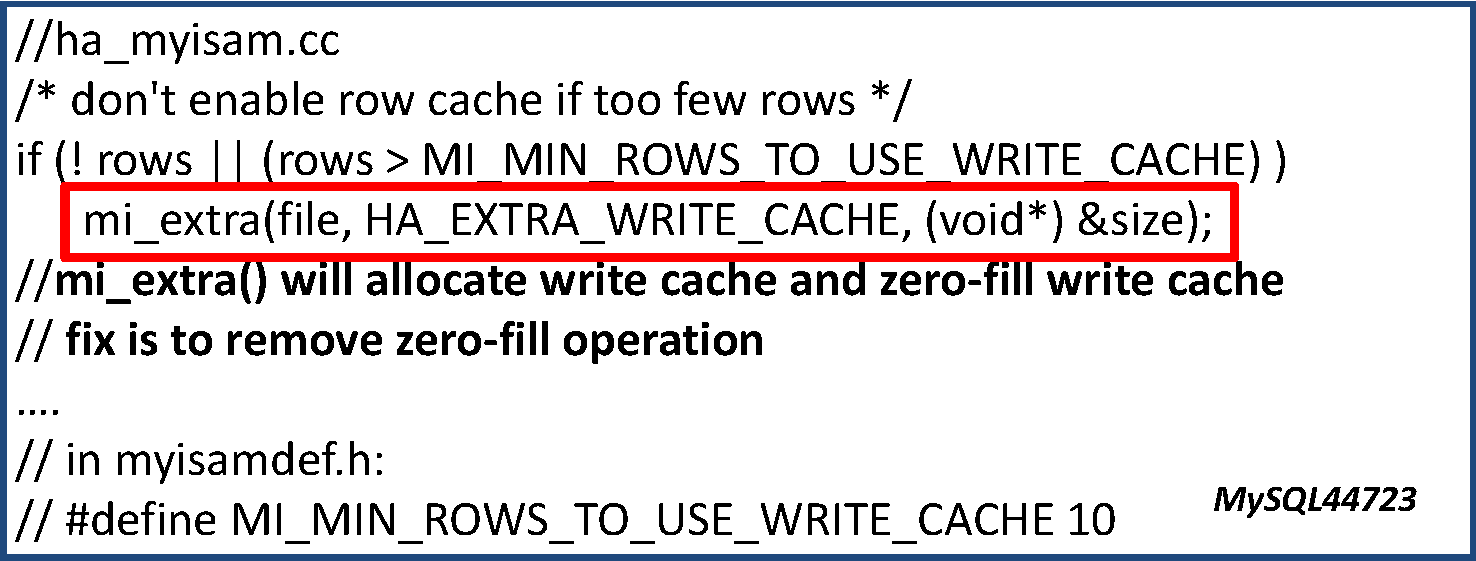
\includegraphics[width=3in]{figures/MySQL44723}
\caption{A MySQL bug diagnosed by Branch}
\label{fig:MySQL44723}
\end{center}
\end{figure}
}


\begin{figure}
\centering
\lstinputlisting[basicstyle=\ttfamily\footnotesize,numbers=left]{figures/MySQL44723.c}
\caption{A MySQL bug diagnosed by Branch}
\label{fig:MySQL44723}
\end{figure}

In most cases, the failure predictor
is very close to the final patch of the performance problem (within 10 lines
of code).
For example, the patch for the Apache bug in Figure 
\ref{fig:Apache3278} is only two lines away from the failure predictor.
As another example, 
the top-ranked failure predictor for the MySQL bug shown in 
Figure \ref{fig:MySQLintro} is at the \lstinline{if(!rows)} branch, and
the patch exactly changes that branch. 




There are also two cases, where the failure predictor is highly related to the
root cause but is in different files from the final patch.
For example, Figure~\ref{fig:MySQL44723} illustrates the performance problem
reported in MySQL\#44723.
MySQL44723 is caused by unnecessarily zero-filling the write cache. 
Users noticed that there is a huge performance difference between 
inserting 9 rows of data and 11 rows of data.
Our statistical debugging points out that the failure is highly
related to taking the
\texttt{(row > MI\_MIN\_ROWS\_TO\_USE\_WRITE\_CACHE)} branch.
That is, success runs never take this branch, yet failure runs always
take this branch.
This is related to the root cause --- an inefficient implementation
of function \texttt{mi\_extra}, and the patch makes \texttt{mi\_extra}
more efficient.

Note that identifying the correct failure predictor is not trivial.
As shown by the ``\# of candidate predicates'' column
of Table \ref{tab:in-house}, there is a large number of predicates that
have been observed true for at least once in failure runs.
Statistical debugging is able to identify the most failure predicting ones
out of thousands or even hundreds of thousands of candidate predicates.

\begin{table*}[tb!]
\begin{adjustwidth}{-.5in}{-.5in}
\small
\centering
{
\begin{tabular}{|lcccccc|}
\hline
&Apache&Chrome&GCC&Mozilla&MySQL&Total\\
\hline
Total \# of bugs  & 16 & 5 & 9 & 19 & 16 & 65 \\
\hline
\multicolumn{7}{|c|}{\bf \# of bugs the default CBI model can help}\\
\multicolumn{1}{|l}{{ Branches} }
&1&0&2&5&5&13\\
\multicolumn{1}{|l}{{ Returns} }
&1&0&0&0&1&2\\
\multicolumn{1}{|l}{{ Scalar-Pairs} }
 &0&0&0&0&0&0\\
\hline
\multicolumn{7}{|c|}{\bf \# of bugs $\Delta$LDA model can help}\\
\multicolumn{1}{|l}{{ Branches$_{\text{loop}}$} }
&10&4&7&12&10&43\\
\multicolumn{1}{|l}{{ Returns} }
%\multicolumn{1}{|l}{{ Returns$>$Branches} }
&0 &0&0& 0&0&0\\
%\multicolumn{1}{|l}{{ Returns$==$Branches} }
%&9&2&4&5&5&25\\
%\multicolumn{1}{|l}{{ Returns$<$Branches} }
%&1&2&1&6&3&13\\
\multicolumn{1}{|l}{{ Scalar-Pairs} }
%\multicolumn{1}{|l}{{ Scalar-Pairs$>$Branches} }
&0 &0&0&0 &0&0\\
%\multicolumn{1}{|l}{{ Scalar-Pairs$==$Branches} }
%&9&4&4&12&9&38\\
%\multicolumn{1}{|l}{{ Scalar-Pairs$<$Branches} }
%&1&0&2&0&0&3\\
\hline
\multicolumn{7}{|c|}{\bf \# of bugs above designs cannot help}\\
\multicolumn{1}{|l}{{ } }
&4&1&0&2&0&7 \\
\hline
\end{tabular}
}
\end{adjustwidth}
\caption{How different predicates work for diagnosing user-reported performance bugs (In this manual inspection, if more than one 
predicate can help diagnose a problem, we only count the predicate
that is most directly related to the root cause)}
\label{tab:predicate}
\end{table*}

\paragraph{Comparing with the profiler}
For eight cases where the basic statistical model is useful, profilers fail miserably. 
In terms of identifying root causes (i.e., what causes the inefficient 
computation), among these 8 cases,
the root-cause functions are ranked from number 11 to 
number 1037 for 5 cases. In the other 3 cases, the
function that contains the root cause does not even appear in the profiling 
result list (i.e., these functions execute for such a short amount of time that
they are not even observed by profilers).

Even if we consider functions in the call stacks of top-ranked
profiler functions, profiler is helpful for only one out of these eight cases,
as shown by the ``Stack'' column of Table \ref{tab:in-house}. That is, for
MySQL44723, the root cause function is the caller's caller of the top ranked
function in profiler results. For the other seven benchmarks, the root
cause functions do not appear on the call stacks of the top five ranked 
functions in profile results.




In terms of suggesting fix strategies, profiler results provide no hint
about how to solve the performance problem. Instead, the statistical debugging
results are informative.
For example, among the 7 cases where branch predicates are 
best failure predictors, the fixes either directly change the branch condition 
(5 cases) or optimize the code in the body of the branch (2 cases).
For the one case where a return predicate is the best failure predictor,
the fix affects the return value of the corresponding function.


\subsubsection{Results for $\Delta$LDA model}
\label{sec:deltalda_results}


\input section/5_delta-lda




\subsection{Manual inspection}
\label{sec:manual_results}

In addition to the above experimental study, we also manually checked
which predicate, if any, would help diagnose each of the 65 user-reported
performance bugs in our benchmark set. The result is shown in 
Table~\ref{tab:predicate}. 

Assuming the basic statistical model,  
traditional predicates (i.e., branches, returns, and scalar-pairs) 
can diagnose 15 out of 65 performance 
problems. Among them,
branch predicates are the most helpful, able to diagnose 13 performance 
problems; return predicates can diagnose 2 performance problems; 
scalar-pair
predicates are the least useful among the three in our study.




Among the ones that cannot be diagnosed by the basic statistical model,
43 of them are caused by inefficient loops. We expect that the 
$\Delta$LDA statistical model can identify root-cause related branch predicates
(denoted as ``Branches$_{\text{loop}}$'' in Table~\ref{tab:predicate}).
That is, the loop-condition branch related to the loop that is executed for too
many times
during failure runs will be ranked high by the $\Delta$LDA model.
Some scalar-pair predicates and function-return predicates could also
help failure diagnosis under the $\Delta$LDA model. For example, the
loop-condition of an inefficient loop could involve the comparison between
two scalar variables; the inefficient loop could invoke a function that
happens to always return positive values; and so on. However, these predicates
will not provide more information than branch predicates. Therefore, we do
not mark them in Table \ref{tab:predicate}.

The remaining 7 performance problems are mostly caused by unnecessary I/Os
or other system calls, not related to any predicates discussed above.

\subsection{Discussion}

Putting our manual inspection results and
experimental evaluation results together, we conclude the following:

\begin{enumerate}
\item Statistical debugging can help the diagnosis of many
user-reported performance problems, improving the state of the art in 
performance diagnosis;

\item Two design points of statistical debugging are particularly useful
for diagnosing performance problems. They are branch predicates under
basic statistical model and branch predicates under $\Delta$LDA model.
These two design points complement each other, providing
\textbf{almost full} coverage of performance problems that we have studied;

\item The basic statistical model that works for most functional bugs
\cite{liblit03,liblit05,tarantula1,tarantula2,tarantula.darko,CCI,joy.asplos13}
is very useful for performance diagnosis too, but still leaves many performance
problems uncovered; statistical models that
consider the number of times a predicate is true 
in each run (e.g., the $\Delta$LDA model)
is needed for diagnosing performance problems.

\item Statistical debugging alone cannot solve all the problem
of diagnosing performance problems. Although statistical debugging
can almost always provide useful information for performance diagnosis, 
developers still
need help to figure out the final patches. Especially, when an inefficient
loop is pointed out by the $\Delta$LDA model, 
developers need more program analysis to understand why the loop is inefficient
and how to optimize it.
\end{enumerate}



To guide future research on performance diagnosis, we further
studied those 43 loop-related performance problems, and manually categorized 
their fix strategies, as shown in
Table \ref{tab:loop-rootcause}.
We expect future performance diagnosis systems to use static or
dynamic analysis to automatically figure out the detailed 
root causes, differentiate effects from causes, and suggest
detailed fix strategies, after statistical debugging identifies
root-cause loop candidates.


%%%%%%%%%%%%%%%%%%%COMMENT OUT%%%%%%%%%%
\comment{
\begin{table*}[tb!]
\begin{adjustwidth}{-.5in}{-.5in}
\small
\centering
{
\begin{tabular}{|c|c|c|c|c|c|c|}
\hline
\multicolumn{1}{|c|}{Predicates} &Apache&Chrome&GCC&Mozilla&MySQL&Total\\
\hline
Total \# of bugs    & 16 & 5 & 9 & 19 & 16 & 65 \\
\hline

Branches                  &1&0&2&5&5&13\\
Returns                  &1&0&0&0&2&3\\
Scalar-Pairs             &0&0&0&0&0&0\\
Loop                    &10&4&7&12&9&42\\
Others                  &4&1&0&2&0&7\\
\hline
\end{tabular}
}
\end{adjustwidth}
\caption{How different predicates work for diagnosing user-perceived performance bugs (manual inspection)}
\label{tab:predicate}
\end{table*}
}

\comment{
\begin{figure}[h!]
\centering
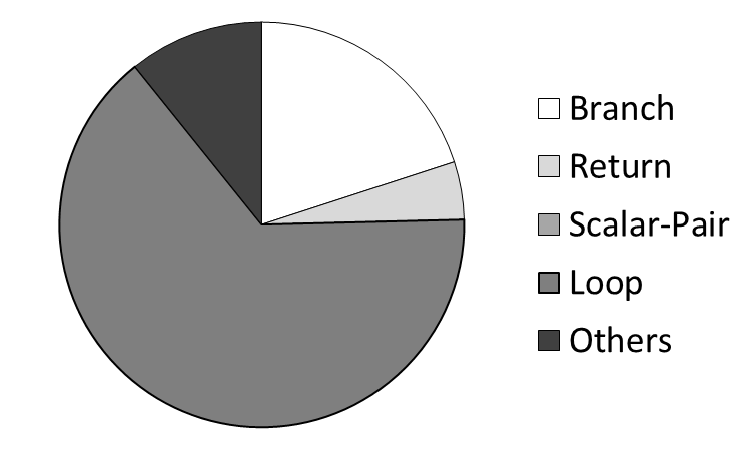
\includegraphics[width=2.5in]{figures/pie}
\caption{How different predicates work for diagnosing user-perceived performance bugs (manual inspection)}
\label{fig:predicate}
\end{figure}
}
